\documentclass[11pt, a4paper]{article}

% --- Ref ---
\usepackage{hyperref}
\hypersetup{hidelinks=true}
\hypersetup{colorlinks=true, linkcolor=blue}
\usepackage[all]{hypcap}

% --- Core Mathematics Packages ---
\usepackage{amsmath}   % Advanced math typesetting (align, matrices, etc.)
\usepackage{amssymb}   % Math symbols (blackboard bold letters like \mathbb{R})
\usepackage{amsthm}    % Theorem environments (theorems, proofs, lemmas)
\usepackage{bm}        % Bold math symbols (\bm{x})

% --- Page Layout & Settings ---
\usepackage[margin=1in]{geometry} % Standard 1-inch margins
\usepackage[utf8]{inputenc}       % Allows special characters directly from keyboard

% --- Theorem Declarations ---
% These define standard environments for mathematical structuring
\newtheorem{theorem}{Theorem}[section]
\newtheorem{lemma}[theorem]{Lemma}
\newtheorem{proposition}[theorem]{Proposition}
\newtheorem{corollary}[theorem]{Corollary}

\theoremstyle{definition}
\newtheorem{definition}[theorem]{Definition}
\newtheorem{example}[theorem]{Example}

\theoremstyle{remark}
\newtheorem*{remark}{Remark}

\usepackage{graphicx} % Required for inserting images

% --- Document Metadata ---
\title{\textbf{EKF for Battery System}}
% \author{}
\date{\today}

% --- Main Document Content ---
\begin{document}

\maketitle

\begin{abstract}
This article will explain what and how the EKF is used and deployed to the actual drone with Ardupilot platform.
\end{abstract}

\section{Battery Model}

\subsection{State}

\begin{align}
    SOC(k+1) &= SOC(k) + \frac{dt}{Q_{nom}}(I(k) + w(k)), \label{eq:orig_soc} \\
    i_{bv}(k+1) &= \frac{\tau}{\tau + \Delta t}i_{bv}(k) + \frac{\Delta t}{\tau + \Delta t} (I(k) + w(k)) \label{eq:orig_ibv}
\end{align}


\subsection{Output}

\begin{align}
    v_{cell}(k) = OCV(SOC(k)) + R_{ac}I(k) + R_{bv}i_{bv}(k) + v(k) \label{eq:orig_volt}
\end{align}

\section{EKF}

\subsection{Linearization}

\begin{align}
    \begin{bmatrix}
        SOC(k+1) \\
        i_{bw}(k+1)
    \end{bmatrix}
    &= 
    \begin{bmatrix}
        1 & 0 \\
        0 & \frac{\tau}{\tau+\Delta t}
    \end{bmatrix}
    \begin{bmatrix}
        SOC(k) \\
        i_{bw}(k)
    \end{bmatrix}
    +
    \begin{bmatrix}
        \frac{dt}{Q_{nom}}\\
        \frac{\Delta t}{\tau + \Delta t}
    \end{bmatrix}
    (I(k)+w(k)), \label{eq:linear_state} \\
    \begin{bmatrix}
        v_{cell}(k)
    \end{bmatrix}
    &=
    \begin{bmatrix}
        \frac{dOCV}{dSOC}(k) & R_{bv}
    \end{bmatrix}
    \begin{bmatrix}
        SOC(k) \\
        i_{bw}(k)
    \end{bmatrix}
    +
    \begin{bmatrix}
    R_{ac}
    \end{bmatrix}
    I(k)
    +
    v(k) \label{eq:linear_output}
\end{align}

\subsection{Error System}


According to \eqref{eq:linear_state}, and \eqref{eq:linear_output}, let

\begin{align}
    x &= \begin{bmatrix}
        SOC &
        i_{bv}
    \end{bmatrix}^{T}, \quad u = \left[ I \right]^{T}, \quad y = \left[ v_{cell} \right]^{T} \\
    A &= \begin{bmatrix}
        1 & 0 \\
        0 & \frac{\tau}{\tau+\Delta t}
    \end{bmatrix} \\
    B_{u} &= B_{w} = \begin{bmatrix}
        \frac{dt}{Q_{nom}}\\
        \frac{\Delta t}{\tau + \Delta t}
    \end{bmatrix} \\
    C &= \begin{bmatrix}
        \frac{dOCV}{dSOC} & R_{bv}
    \end{bmatrix} \\
    D_{u} &= \begin{bmatrix}
        R_{ac}
    \end{bmatrix}, \quad D_{v} = \begin{bmatrix}
        1
    \end{bmatrix}
\end{align}

System can be represent as this,

\begin{align}
    x(k+1) = Ax(k) + B_{u}u(k) + B_{w}w(k), \\
    y(k) = Cx(k) + D_{u}u(k) + D_{v}v(k)
\end{align}

The estimated model is
\begin{align}
    \hat{x}(k+1) = A\hat{x}(k) + B_{u}u(k), \\
    \hat{y}(k) = C\hat{x}(k) + D_{u}u(k)
\end{align}

Then the error system should be,
\begin{align}
    \tilde{x}(k+1) &= A\tilde{x}(k) + B_{w}w(k), \\
    \tilde{y}(k) &= C\tilde{x}(k) + D_{v}v(k)
\end{align}

This should be the system for EKF.

\section{Result}

\begin{figure}[htbp]
    \centering
    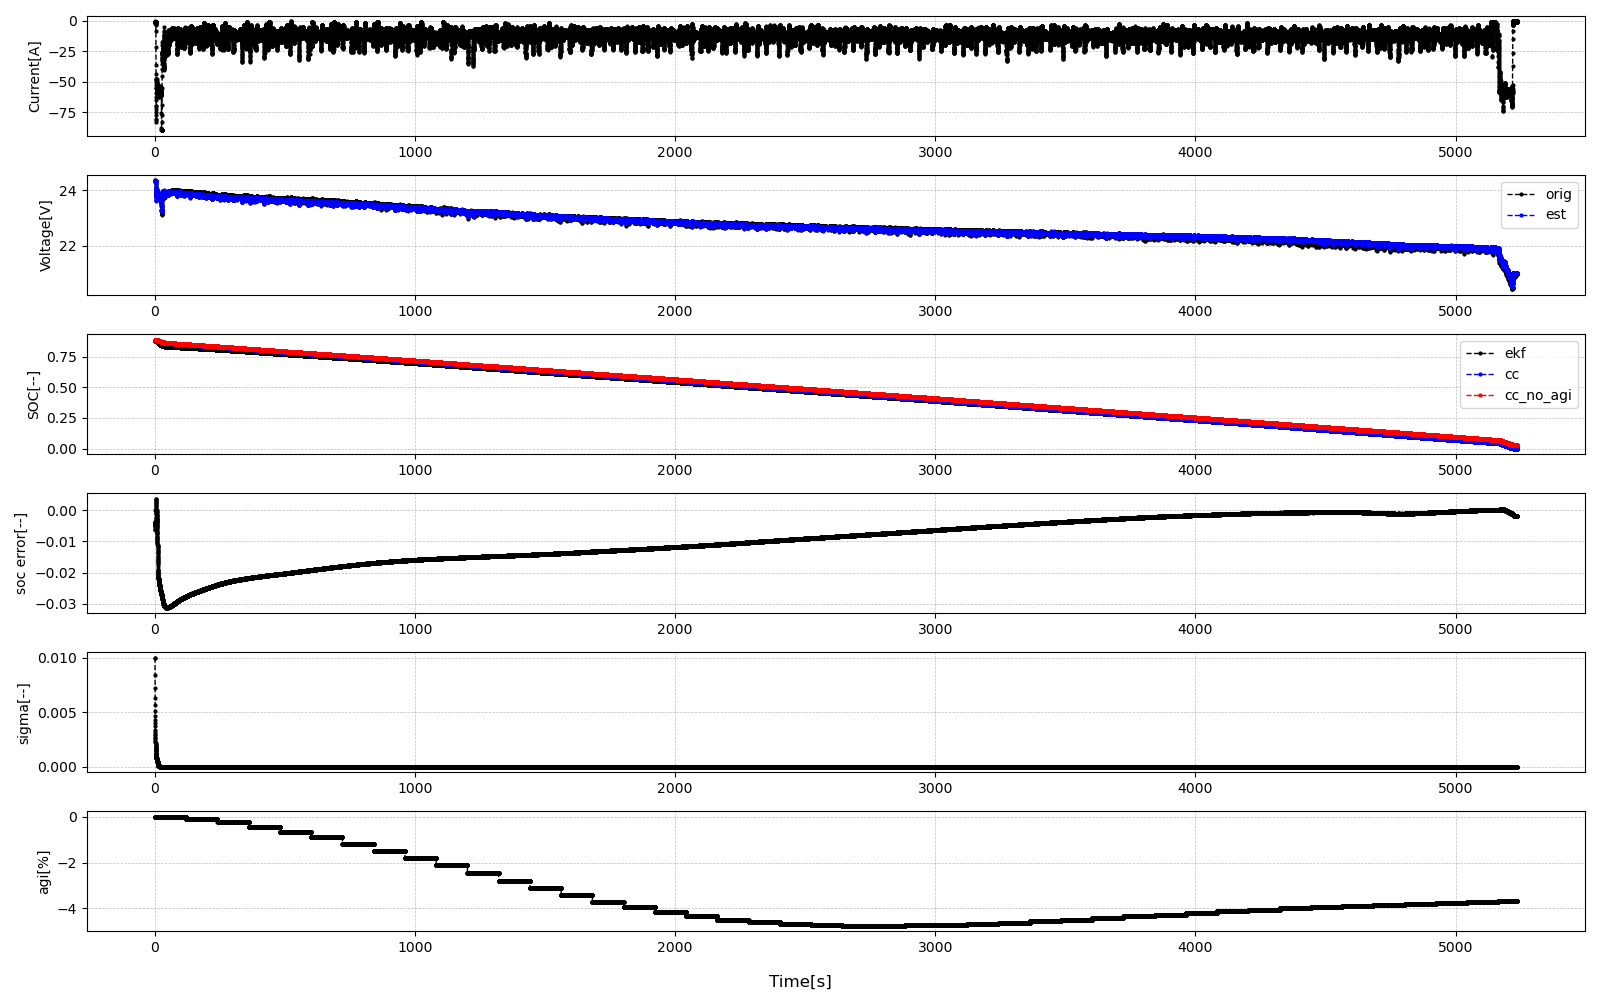
\includegraphics[width=1.0\textwidth]{../test/result/EKF.png}
    \caption{Result of flight test.}
    \label{fig:EKF}
\end{figure}

\begin{figure}[htbp]
    \centering
    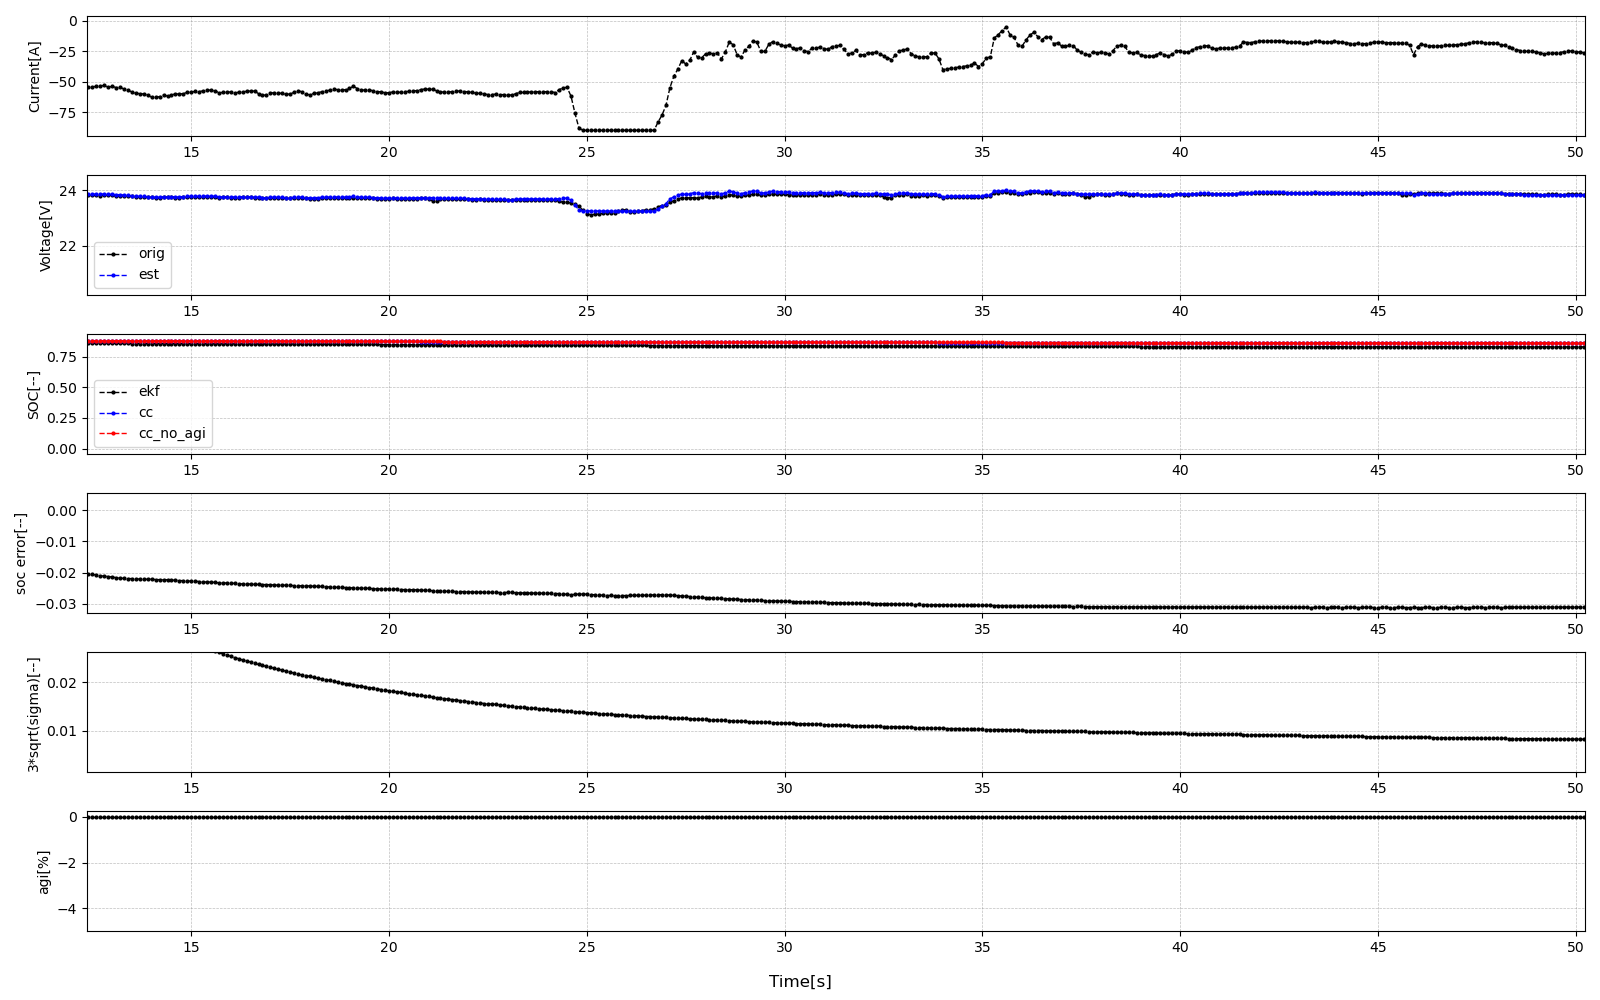
\includegraphics[width=1.0\textwidth]{../test/result/EKF_first20sec.png}
    \caption{Convergence of sigma value for SOC estimation error.}
    \label{fig:EKF_first20sec}
\end{figure}

    Figure \ref{fig:EKF} is the full trajectory of current, voltage, SOC, and SOH.
    The battery is around 3.2\% less than the total capacity tested (21.671 Ah).
    The EKF estimate SOC with the 21.671 Ah and manage to track the actual SOC shown in blue.

    Figure \ref{fig:EKF_first20sec} shows the convergence of the error $\tilde{x}=x-\hat{x}$.
    The $3\sqrt{\sigma(\tilde{x})} \le 0.02$ after 20 seconds, which shows the confidence of the estimation.

\end{document}
